\chapter{Goals}
Our goal is to develop a graphical editor for music generation. With it's help it will be possible to create patches, test their output in a simulation and produce a netlist to generate that sound on a \ac{FPGA}. A patch can be build with different sound-components like wave generators and filters. In order to create specific sounds, the sound-components have to be connected. The exported netlist can be put on a \ac{FPGA} so the user of the synthesizer (e.g. a musician) can connect a MIDI device or specific sensors to the \ac{FPGA} to modify input values at runtime. \\
To describe the functions, which we want to develop, in detail, we provide use case diagrams.

\section{Editor for the designer}
\label{editor}
Figure \ref{fig:Soundgate_Designer} shows the use cases for the editor.

	\begin{figure}[!h]
		\centering
			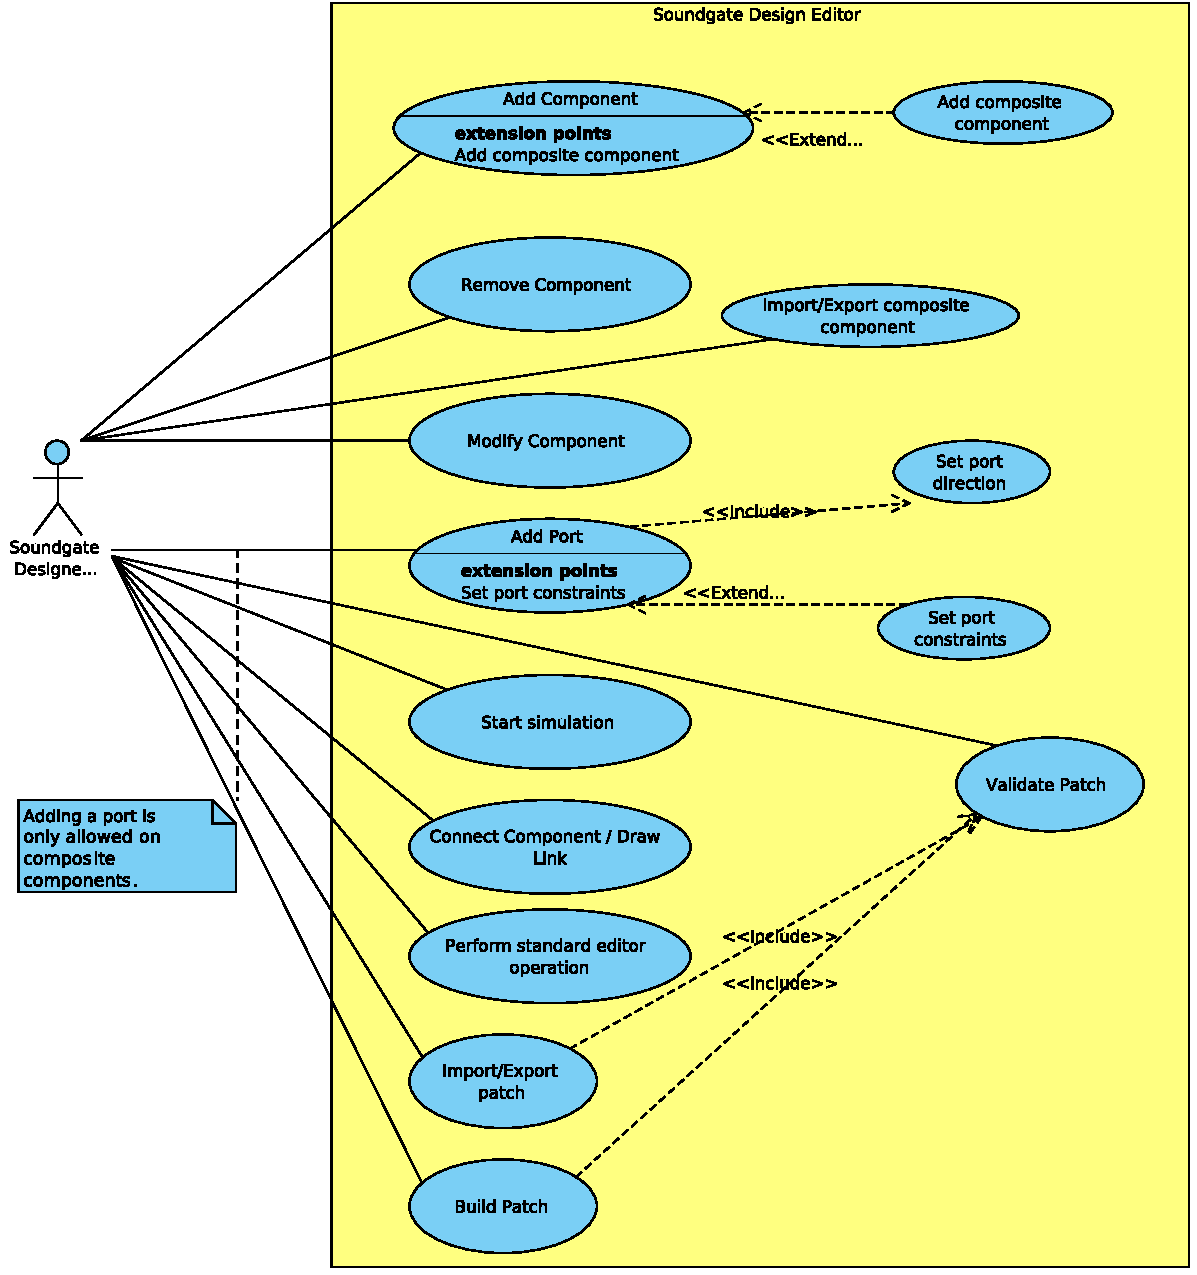
\includegraphics[width=1\textwidth]{images/Soundgate_Designer.pdf}
		\caption{Use case diagram for the Soundgate editor}
		\label{fig:Soundgate_Designer}
	\end{figure}

In the editor the designer can create a new patch, open an existing patch or save his own one. \\
He can add sound-components to the patch and remove them from the patch. He can connect sound-components by drawing links between their ports. A sound-components can be an atomic sound-components like a sound generator, filter etc. The atomic sound-components are stored within XML-libraries; their ports are predefinied. Some of these sound-components have static properties, which the designer can modify (e.g. the value of a constant-block). The other kind of sound-components are composite sound-components. The designer can add a composite sound-components to the patch and fill it on his own with other sound-components and links between them. He can add ports to a composite sound-components and define their direction and constraints. We want to make it possible to export finished composite sound-components as XML-files and to import existing ones to the editor such that different designers can exchange their sound-components.\\
Furthermore, the designer must define the interfaces of his patch. The interfaces are the points where the end-user interacts with the system. These can be MIDI-inpus, sensor values etc.\\
If a patch is finished, it can be validated. The program tests if all constraints are fulfilled (e.g. if all ports are connected and so on). The designer can build it, which means that he can generate VHDL-code out of the XML-file.\\
Of course, all standard editor operations like selecting, moving objects etc. are supported.

\section{Simulator}

We want to develop a software simulator for a patch such that the designer and the user can test the sound of the patch before putting it on a \ac{FPGA}. Figure \ref{fig:Soundgate_Simulator} shows the use cases for the Soundgate simulator.

	\begin{figure}[!h]
		\centering
			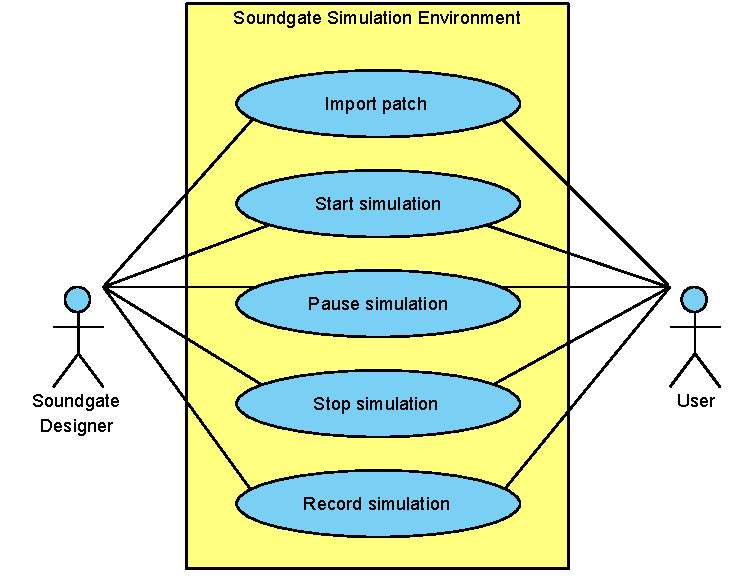
\includegraphics[width=0.90\textwidth]{images/Soundgate_Simulator.pdf}
		\caption{Use case diagram for the Soundgate simulation environment}
		\label{fig:Soundgate_Simulator}
	\end{figure}

A designer must be able to import a patch to the simulator and to start the simulation. Afterwards he is able to pause or stop the simulation. An optional feature we would like to implement is the possibility to save the output of a simulation on the HDD.

\section{COSMIC system}

Figure \ref{fig:Soundgate_UserInterface} shows use cases for the \ac{COSMIC} system.

	\begin{figure}[!h]
		\centering
			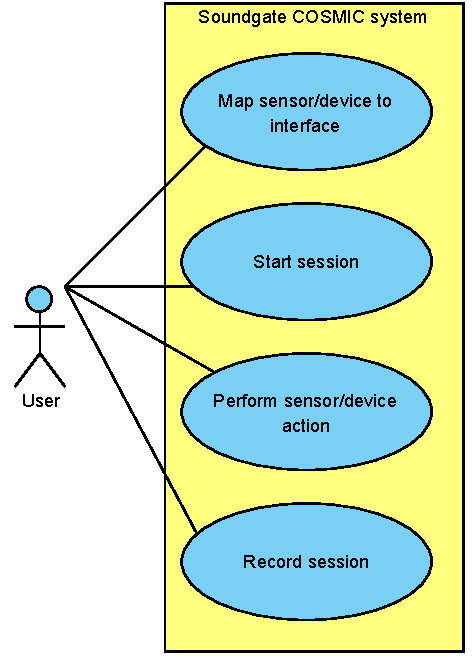
\includegraphics[width=0.50\textwidth]{images/User_View.pdf}
		\caption{Use case diagram of the Soundgate COSMIC system}
		\label{fig:Soundgate_UserInterface}
	\end{figure}
	
	As mentioned before, a patch created in the editor can be exported as a XML-file which is used to generate VHDL-code. This VHDL-code is synthesized and put on a \ac{FPGA}. The end-user (e.g. a musician or a performer) maps sensor values and other inputs to the interfaces defined by the designer (see Sec. \ref{editor}). He starts the session by pushing a button. During the session he performs some sensor actions or actions with other devices to create input values for the system.
	
\subsection{Input}
We will provide different ways of modfiying the patch at runtime through sensors. The first approach uses a device as a sensors whereas the other one will use the body of the musician, which will be tracked by a 3D depth camera. 

\subsubsection{Mobile Device}
Today's mobile phones are full of different sensors which can easily be accessed with a small application. The Android SDK offers three different groups of sensors, namely:
\begin{itemize}
	\item \textbf{Motion Sensors} \\
			This group contains accelerometers, gravity sensors, gyroscope, and rotational vector sensors (TODO see ref to Android page). 
	\item \textbf{Environmental Sensors} \\
			With their help it is possible to check the air temperature illumination and humidity.
	\item \textbf{Position Sensors} \\
			Orientation sensors and magnometers.
\end{itemize}

However, environmental sensors are not suitable since modfiying their values can not be done quickly enough. The other sensors are perfectly suited for changing values since they are modified simply by moving the phone and changing it's orientation. We will develop an Android Application because the Android OS is widespred. On the one hand the sensors have to be read by the application and on the other hand these values have to be forwared to the simulation environment. This can be done with Sockets to send these values over a network connection.

\subsubsection{3D depth camera}
A 3D camera like the Microsoft Kinect system is able to calculate the depth of an image. Therefore it is possible to track the movement of a person by tracking different joints, which have to be calibrated at the beginning. So it is possible to connect parametes of a sound component i.e. the altitude, to one of the person's arms. This method abstracts the sensors so it feels like if the person himself is possible to change the sound.

Furthermore the end-user should be able to use MIDI devices.

\section{Open Sound Control}
The communication between the sensors and the entire system will be made through ethernet and WiFi. Therefore it is possible to send different values to the \ac{FPGA} so it changes it's parameters. Through ReconOS and a Linux kernel it is possible to open a server socket to listen for those messages. However it is necessary to agree on a specific protocol. Instead of developing an own protocol, we are going to use the Open Sound Control Protocol. \\
The OSC is a message based communication protocol. Signals can be created by the different sensors and send to the receiver. Additionally it is not transport protocol dependent, so we could either use error detecting TCP or the faster UDP protocol. Since a device is capable of generating a relative big amount of data per second, we are most likely forced to use UDP. If there is any packet loss or transmission error it will not be detected. However the user usually would not hear this (omfg überarbeite mich).  
\begin{itemize}
\item{OSC message}
\begin{itemize}
\item{1 Byte contains length of packet and the rest data. length = $2^x$}
\item{datatypes: int32, float32, OSCString, OSCTimetag, OSCBlob}
\end{itemize}
\end{itemize}

\section{Component library}
We plan to provide following components:

\begin{itemize}
\item Generators:
\begin{itemize}
\item Sinus
\item Sawtooth
\end{itemize}

\item Filters:
\begin{itemize}
\item Ramp
\item Low pass
\item Delay
\end{itemize}

\item Arithmetic:
\begin{itemize}
\item Addition 
\item Multiplication
\item Equals
\end{itemize}

\item Mixer

\item Sources:
\begin{itemize}
\item Constant
\end{itemize}

\item Sinks:
\begin{itemize}
\item Sound output
\end{itemize}

\item MIDI: 
\begin{itemize}
\item MIDI note to frequency converter
\item MIDI scheduler
\end{itemize}

\end{itemize}